\begin{center}
    \textbf{ВВЕДЕНИЕ}
\end{center}
\addcontentsline{toc}{chapter}{ВВЕДЕНИЕ}




Многопоточность --- способность центрального процессора или одного ядра в
многоядерном процессоре одновременно выполнять несколько процессов или
потоков, соответствующим образом поддерживаемых операционной системой.

Потоки --- это задача виртуального процессора, точно так же, как
виртуальный процессор является задачей ЦПУ. Потоки иногда называют
облегченными процессами, так как они похожи на процессы, но предъявляют
меньше требований к операционной системе \cite{bib0}.




\textbf{Цель лабораторной работы} --- Получить навык организации параллельных
вычислений на основе нативных потоков.

Для достижения поставленной цели необходимо выполнить следующие задачи:
\begin{itemize}
    \item разработка алгоритма обработки данных;
    \item создание ПО, реализующего разработанный алгоритм;
    \item исследование характеристик созданного ПО.
\end{itemize}


\section{Входные данные}
Входными данными программы является URL ссылка пагинации.


\section{Выходные данные}
Выходные данные --- директория с файлами, которые содержат скачанные данные
со страниц параграфы.

\clearpage

\section{Тестирование}
В таблице \ref{tbl:time_measurements} представлены функциональные тесты для разработанного
программного обеспечения. Все тесты пройдены успешно.


\begin{table}[h]
	\begin{center}
		\begin{threeparttable}
		\captionsetup{justification=raggedright,singlelinecheck=off}
		\caption{Время работы алгоритмов (в секундах)}
		\label{tbl:time_measurements}
                        \begin{tabular}{|p{4cm}|p{4cm}|p{4cm}|p{4cm}|}
                            \hline
                            № Теста & Входные данные & Полученные \ данные & Ожидаемые выходные данные \\
                            \hline
                            1 & https://vkusnye-recepty.ru/page/ & Директория с текстами рецептов &
                            Директория с текстами рецептов \\
                            \hline
                            2 & https://nevkusnye-recepty.ru/page/ --- несуществующая ссылка
                              & Error. Invalid URL: https://nevkusnye-recepty.ru/page/1 &
                            Error. Invalid URL: https://nevkusnye-recepty.ru/page/1 \\
                            \hline
                            3 &  & Error. Invalid URL: 1 &
                            Error. Invalid URL: 1 \\
                            \hline

                        \end{tabular}
		\end{threeparttable}
    \end{center}
\end{table}

\section{Исследование}
В ходе исследования требуется получить характеристики созданного ПО в зависимости
от количества потоков или от количеста обрабатываемых страниц сайта.

\subsection{Технические характеристики}
Технические характеристики устройства, на котором выполнялось тестирование:
\begin{itemize}
    \item Операционная система: Linux \cite{bib1};
    \item Память: 16 GB;
    \item Процессор: AMD Ryzen 7 5800H \cite{bib2, bib3}.
\end{itemize}

\subsection{Исследование характеристик}

В таблице \ref{tbl:time_measurements1} приведено время выполнения
программного обеспечения в миллисекундах (далее --- мс). На рисунке
\ref{fig:image1} показана зависимость времени работы от количества
потоков без изменений количества обрабатываемых страниц сайта.

\begin{table}[h]
	\begin{center}
		\begin{threeparttable}
		\captionsetup{justification=raggedright,singlelinecheck=off}
		\caption{Время работы от количества потоков (в миллисекундах)}
		\label{tbl:time_measurements1}
                    \begin{tabular}{|r|r|}
                        \hline
                        Количество потоков & Время работы\\
                        \hline
                        1 & 4494.6 \\
                         \hline
                        2 & 2449.4 \\
                         \hline
                        4 & 1862.2 \\
                         \hline
                        8 & 1407.6 \\
                         \hline
                        16 & 930.8 \\
                         \hline
                        32 & 385.4 \\
                         \hline
                        64 & 185.4 \\
                         \hline
                    \end{tabular}
		\end{threeparttable}
    \end{center}
\end{table}

\begin{figure}[h!]
    \centering
    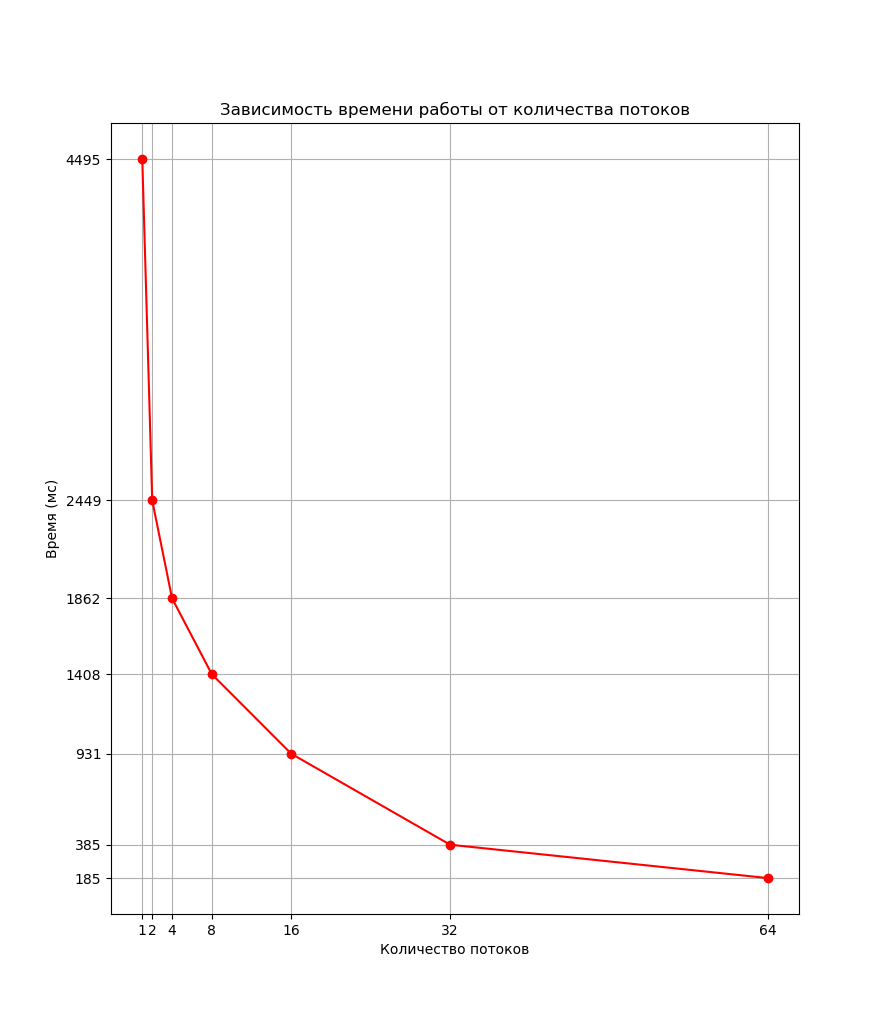
\includegraphics[width=0.8\textwidth]{images/image1}
    \caption{Исследование характеристик созданного ПО от количества потоков}
    \label{fig:image1}
\end{figure}


\clearpage

В таблице \ref{tbl:time_measurements2} приведено время выполнения в зависимости
от количества обрабатываемых страниц. В отличие от предыдущего исследования,
в таблице \ref{tbl:time_measurements2} отсутствует зависимость от количества
потоков.

\begin{table}[h]
	\begin{center}
		\begin{threeparttable}
		\captionsetup{justification=raggedright,singlelinecheck=off}
		\caption{Время работы в зависимости от количества обрабатываемых страниц (в миллисекундах)}
		\label{tbl:time_measurements2}
                \begin{tabular}{|r|r|r|}
			\hline 
			& \multicolumn{2}{c|}{Время для реализации} \\
                        \cline{2-3}
			Количество страниц & 16-поточного & 1-поточного\\
			\hline
                        1 & 215.0 & 3437.4 \\
                         \hline
                        2 & 716.4 & 10615.8 \\
                         \hline
                        3 & 1372.6 & 21063.4 \\
                         \hline
                        4 & 2222.2 & 34714.6 \\
                         \hline
                        5 & 2821.6 & 46838.5 \\
                         \hline
		\end{tabular}
		\end{threeparttable}
    \end{center}
\end{table}

На рисунке \ref{fig:image2} показана зависимость времени работы от количества
обрабатываемых страниц.

\begin{figure}[h!]
    \centering
    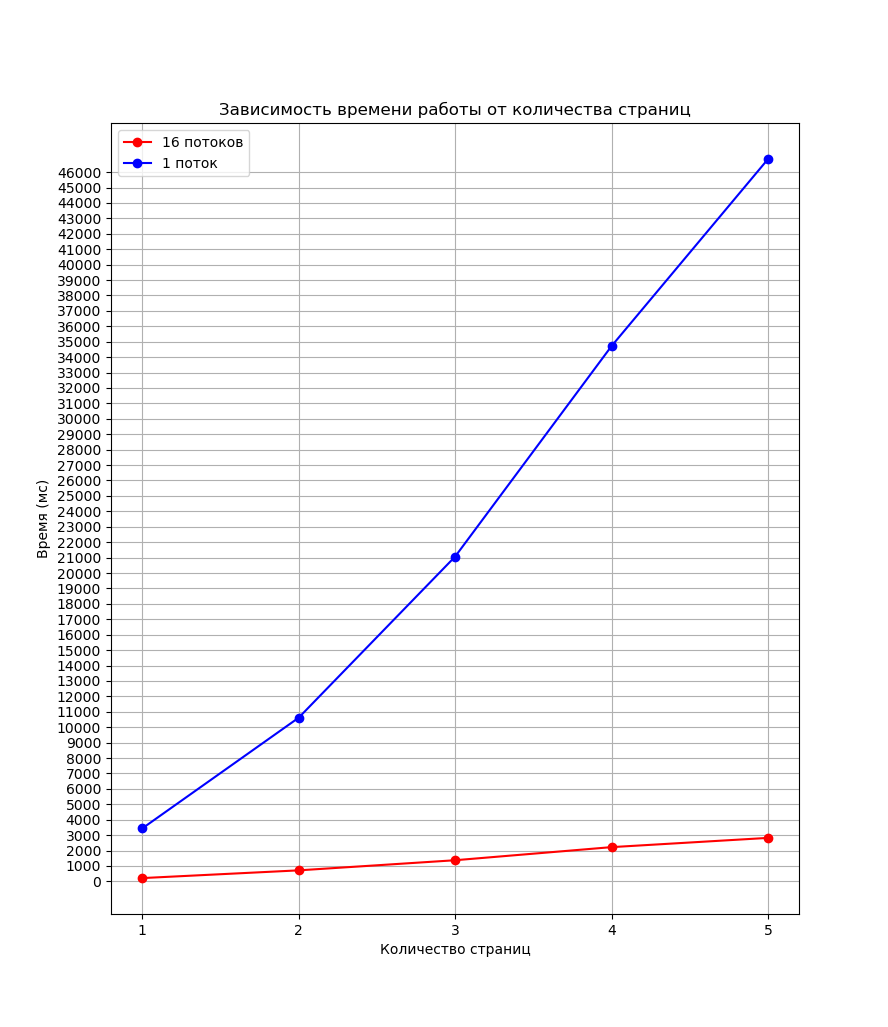
\includegraphics[width=0.8\textwidth]{images/image2}
    \caption{Исследование характеристик созданного ПО от количества обрабатываемых страниц}
    \label{fig:image2}
\end{figure}

\clearpage

\paragraph*{ВЫВОД} ${}$ \newline

По результатам проведенного исследования можно сказать, что время работы
однопоточной реализации работа программы медленнее, чем в многопоточной
реализации программы. Так, при фиксированном количестве потоков и при изменяющемся
количестве обрабатываемых страниц время выполнения однопоточной реализации программы
уступает в 16-17 раз по времени выполнения 16-поточной программы.

При росте количества потоков и при фиксированном количестве обрабатываемых
страниц время выполнения
уменьшается в 1.5-2.5 раза при увеличением количества потоков в два раза.
Самая большая разница во времени выполнения между двух поточной программой
и однопоточной программой, время выполнения которых различается в 1.8 раз. 


\begin{center}
    \textbf{ЗАКЛЮЧЕНИЕ}
\end{center}
\addcontentsline{toc}{chapter}{ЗАКЛЮЧЕНИЕ}

Цель работы достигнута. Решены все поставленные задачи:
\begin{itemize}
    \item разработка алгоритма обработки данных;
    \item создание ПО, реализующего разработанный алгоритм;
    \item исследование характеристик созданного ПО.
\end{itemize}




